\documentclass{standalone}
\usepackage{tikz}
\usetikzlibrary{patterns, positioning}
\usepackage[sfdefault]{ClearSans} %% option 'sfdefault' activates Clear Sans as the default text font
\usepackage[T1]{fontenc}

\begin{document}
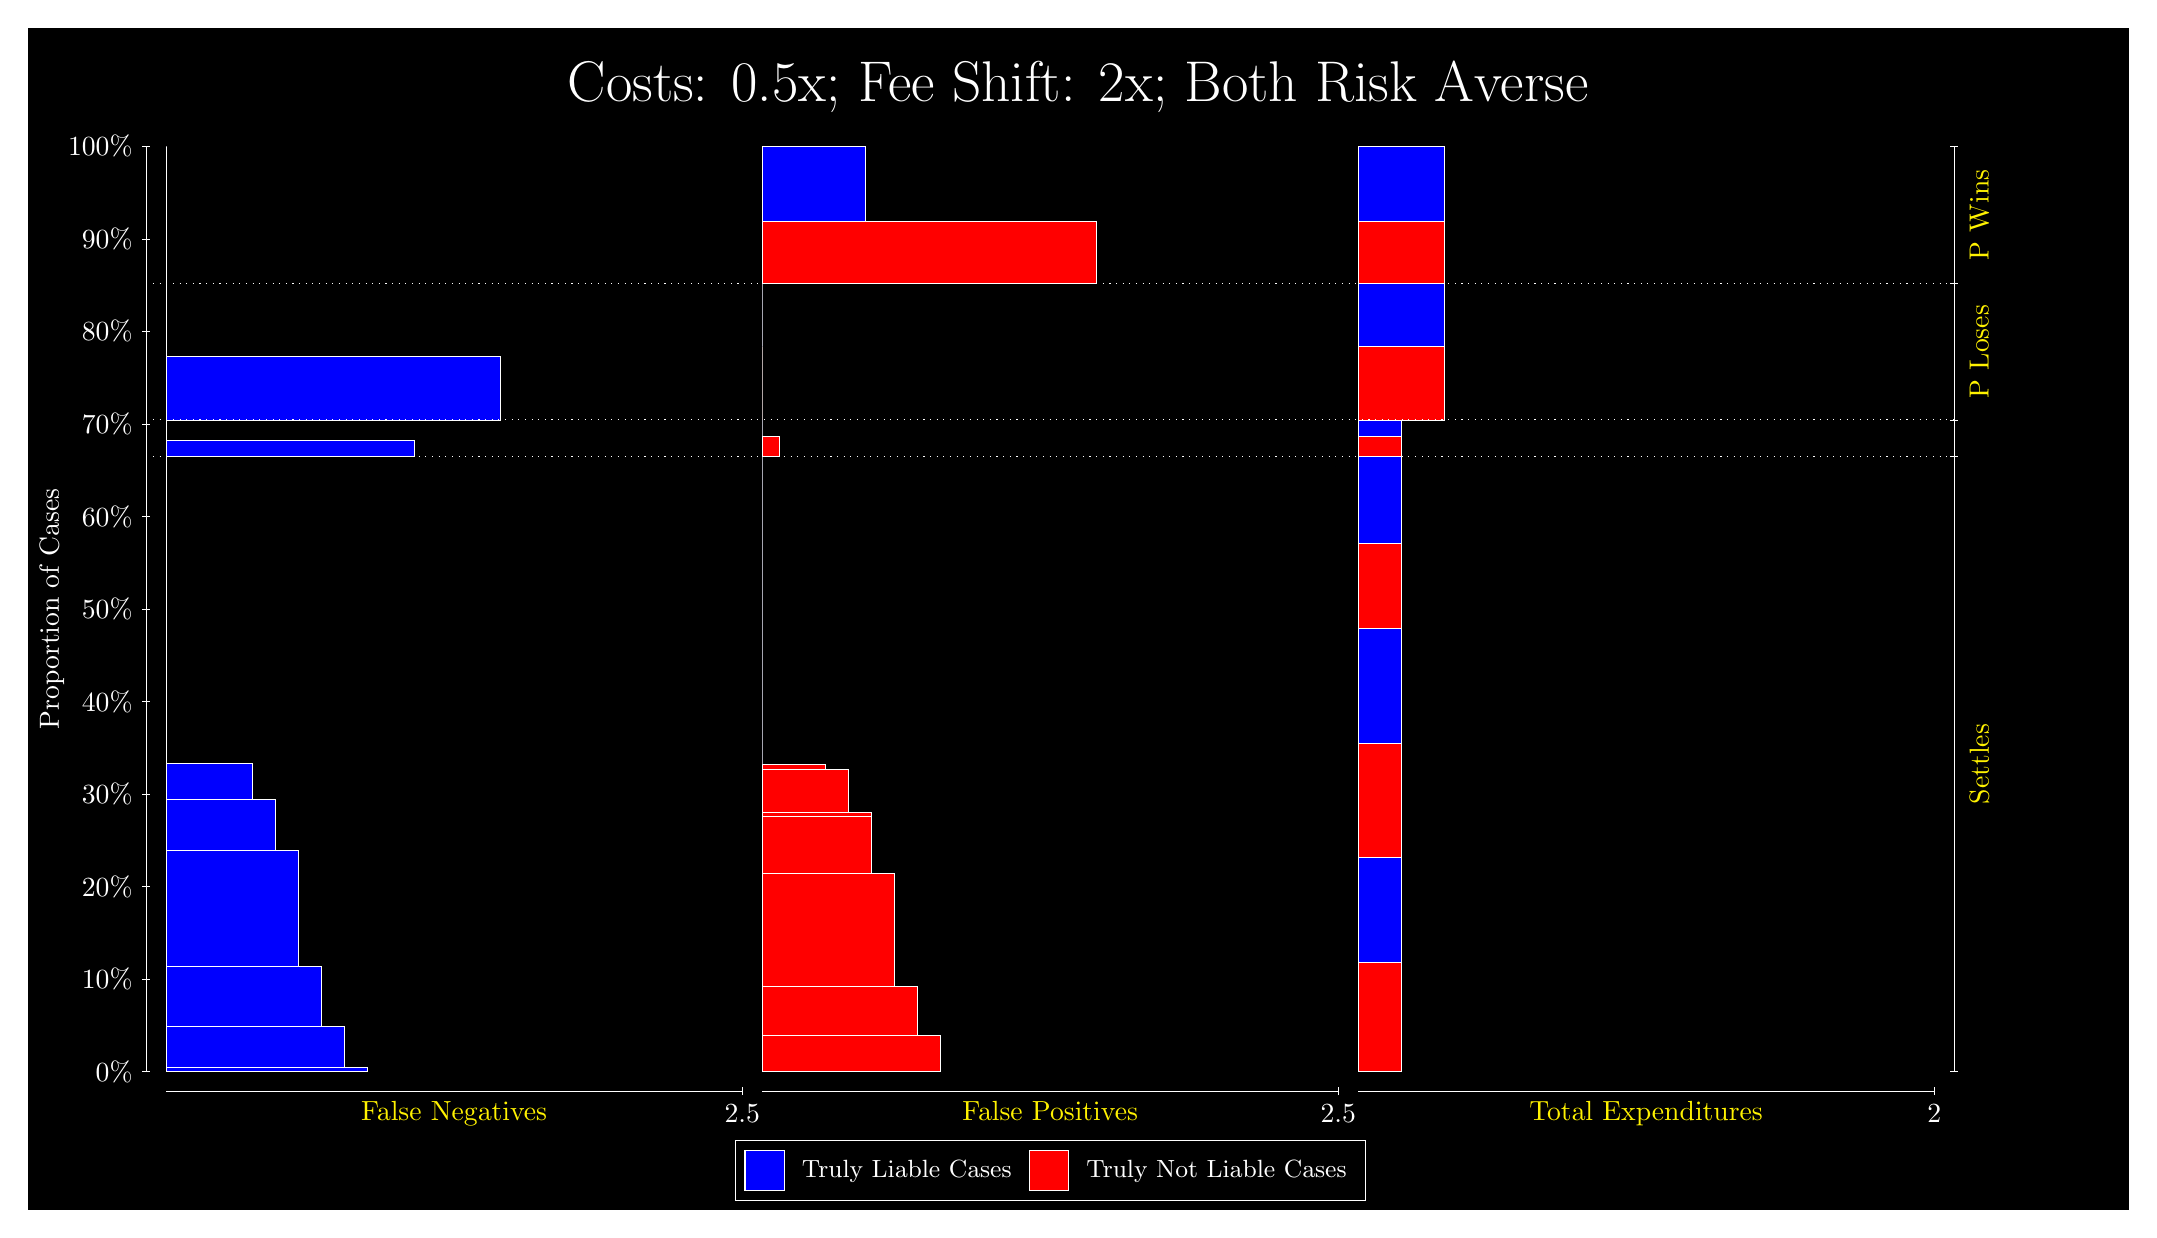
\begin{tikzpicture}
\draw[fill=black] (0,0) rectangle (26.667,15);
\draw[text=white] (0,13.5) rectangle (26.667,15) node[midway] {\huge Costs: 0.5x; Fee Shift: 2x; Both Risk Averse};
\draw[white, very thin] (1.5,1.75) -- (1.5,13.5);
\node[rotate=90, text=white, anchor=center] at (0.3, 7.625) {Proportion of Cases};
\draw[white, very thin] (1.45,1.75) -- (1.55,1.75);
\node[text=white, anchor=east] at (1.45, 1.75) {0\%};
\draw[white, very thin] (1.45,2.925) -- (1.55,2.925);
\node[text=white, anchor=east] at (1.45, 2.925) {10\%};
\draw[white, very thin] (1.45,4.1) -- (1.55,4.1);
\node[text=white, anchor=east] at (1.45, 4.1) {20\%};
\draw[white, very thin] (1.45,5.275) -- (1.55,5.275);
\node[text=white, anchor=east] at (1.45, 5.275) {30\%};
\draw[white, very thin] (1.45,6.45) -- (1.55,6.45);
\node[text=white, anchor=east] at (1.45, 6.45) {40\%};
\draw[white, very thin] (1.45,7.625) -- (1.55,7.625);
\node[text=white, anchor=east] at (1.45, 7.625) {50\%};
\draw[white, very thin] (1.45,8.8) -- (1.55,8.8);
\node[text=white, anchor=east] at (1.45, 8.8) {60\%};
\draw[white, very thin] (1.45,9.975) -- (1.55,9.975);
\node[text=white, anchor=east] at (1.45, 9.975) {70\%};
\draw[white, very thin] (1.45,11.15) -- (1.55,11.15);
\node[text=white, anchor=east] at (1.45, 11.15) {80\%};
\draw[white, very thin] (1.45,12.325) -- (1.55,12.325);
\node[text=white, anchor=east] at (1.45, 12.325) {90\%};
\draw[white, very thin] (1.45,13.5) -- (1.55,13.5);
\node[text=white, anchor=east] at (1.45, 13.5) {100\%};

\draw[white, very thin] (24.457,1.75) -- (24.457,13.5);
\draw[white, very thin] (24.407,1.75) -- (24.507,1.75);
\node[anchor=west] at (24.407, 1.75) {};
\draw[white, very thin] (24.407,9.5585) -- (24.507,9.5585);
\node[anchor=west] at (24.407, 9.5585) {};
\draw[white, very thin] (24.407,10.027) -- (24.507,10.027);
\node[anchor=west] at (24.407, 10.027) {};
\draw[white, very thin] (24.407,11.761) -- (24.507,11.761);
\node[anchor=west] at (24.407, 11.761) {};
\draw[white, very thin] (24.407,13.5) -- (24.507,13.5);
\node[anchor=west] at (24.407, 13.5) {};

\draw[white, very thin, fill=blue] (1.75,1.75) rectangle (4.3116,1.7978);
\draw[white, very thin, fill=blue] (1.75,1.7978) rectangle (4.0188,2.3242);
\draw[white, very thin, fill=blue] (1.75,2.3242) rectangle (3.7261,3.0928);
\draw[white, very thin, fill=blue] (1.75,3.0928) rectangle (3.4333,4.5617);
\draw[white, very thin, fill=blue] (1.75,4.5617) rectangle (3.1406,5.2044);
\draw[white, very thin, fill=blue] (1.75,5.2044) rectangle (2.8478,5.6606);
\draw[white, very thin, fill=red] (1.75,5.6606) rectangle (1.75,9.5585);
\draw[white, very thin, fill=blue] (1.75,9.5585) rectangle (4.8971,9.7697);
\draw[white, very thin, fill=red] (1.75,9.7697) rectangle (1.75,10.027);
\draw[white, very thin, fill=blue] (1.75,10.027) rectangle (5.9949,10.832);
\draw[white, very thin, fill=red] (1.75,10.832) rectangle (1.75,11.761);
\draw[white, very thin, fill=red] (1.75,11.761) rectangle (1.75,12.551);
\draw[white, very thin, fill=blue] (1.75,12.551) rectangle (1.75,13.5);
\draw[white, very thin, fill=red] (9.3189,1.75) rectangle (11.588,2.2044);
\draw[white, very thin, fill=red] (9.3189,2.2044) rectangle (11.295,2.8279);
\draw[white, very thin, fill=red] (9.3189,2.8279) rectangle (11.002,4.2666);
\draw[white, very thin, fill=red] (9.3189,4.2666) rectangle (10.709,4.9871);
\draw[white, very thin, fill=red] (9.3189,4.9871) rectangle (10.709,5.0463);
\draw[white, very thin, fill=red] (9.3189,5.0463) rectangle (10.417,5.5896);
\draw[white, very thin, fill=red] (9.3189,5.5896) rectangle (10.124,5.6479);
\draw[white, very thin, fill=blue] (9.3189,5.6479) rectangle (9.3189,9.5585);
\draw[white, very thin, fill=red] (9.3189,9.5585) rectangle (9.5384,9.8159);
\draw[white, very thin, fill=blue] (9.3189,9.8159) rectangle (9.3189,10.027);
\draw[white, very thin, fill=red] (9.3189,10.027) rectangle (9.3189,10.956);
\draw[white, very thin, fill=blue] (9.3189,10.956) rectangle (9.3189,11.761);
\draw[white, very thin, fill=red] (9.3189,11.761) rectangle (13.564,12.551);
\draw[white, very thin, fill=blue] (9.3189,12.551) rectangle (10.636,13.5);
\draw[white, very thin, fill=red] (16.888,1.75) rectangle (17.437,3.1312);
\draw[white, very thin, fill=blue] (16.888,3.1312) rectangle (17.437,4.4741);
\draw[white, very thin, fill=red] (16.888,4.4741) rectangle (17.437,5.9128);
\draw[white, very thin, fill=blue] (16.888,5.9128) rectangle (17.437,7.3817);
\draw[white, very thin, fill=red] (16.888,7.3817) rectangle (17.437,8.4596);
\draw[white, very thin, fill=blue] (16.888,8.4596) rectangle (17.437,9.5585);
\draw[white, very thin, fill=red] (16.888,9.5585) rectangle (17.437,9.8159);
\draw[white, very thin, fill=blue] (16.888,9.8159) rectangle (17.437,10.027);
\draw[white, very thin, fill=red] (16.888,10.027) rectangle (17.986,10.956);
\draw[white, very thin, fill=blue] (16.888,10.956) rectangle (17.986,11.761);
\draw[white, very thin, fill=red] (16.888,11.761) rectangle (17.986,12.551);
\draw[white, very thin, fill=blue] (16.888,12.551) rectangle (17.986,13.5);
\draw[white, dotted] (1.5,9.5585) -- (24.457,9.5585);
\draw[white, dotted] (1.5,10.027) -- (24.457,10.027);
\draw[white, dotted] (1.5,11.761) -- (24.457,11.761);
\draw[white, very thin] (1.75,1.5) -- (9.0689,1.5);
\node[text=yellow, anchor=north] at (5.4094, 1.5) {False Negatives};
\draw[white, very thin] (9.0689,1.45) -- (9.0689,1.55);
\node[text=white, anchor=north] at (9.0689, 1.45) {2.5};

\draw[white, very thin] (9.3189,1.5) -- (16.638,1.5);
\node[text=yellow, anchor=north] at (12.978, 1.5) {False Positives};
\draw[white, very thin] (16.638,1.45) -- (16.638,1.55);
\node[text=white, anchor=north] at (16.638, 1.45) {2.5};

\draw[white, very thin] (16.888,1.5) -- (24.207,1.5);
\node[text=yellow, anchor=north] at (20.547, 1.5) {Total Expenditures};
\draw[white, very thin] (24.207,1.45) -- (24.207,1.55);
\node[text=white, anchor=north] at (24.207, 1.45) {2};

\node[text=yellow, centered, rotate=90] at (24.777, 5.6543) {Settles};

\node[text=yellow, centered, rotate=90] at (24.777, 10.894) {P Loses};
\node[text=yellow, centered, rotate=90] at (24.777, 12.63) {P Wins};

\draw (12.978300999999998,1.5) node[draw=none] (baseCoordinate) {};
\begin{scope}[align=center]
        \matrix[scale=0.5, draw=white, below=0.5cm of baseCoordinate, nodes={draw}, column sep=0.1cm]{
            \node[rectangle, draw, minimum width=0.5cm, minimum height=0.5cm, fill=blue] {}; &
            \node[draw=none, font=\small, text=white] (B) {Truly Liable Cases}; &
            \node[rectangle, draw, minimum width=0.5cm, minimum height=0.5cm, fill=red] {}; &
            \node[draw=none, font=\small, text=white] (B) {Truly Not Liable Cases}; \\
            };
\end{scope}

\end{tikzpicture}
\end{document}